\section{Sequences}
In this sections the important processes of the system are shown exemplarily. They include a request 
from the web page handled in the web server tier, a call on the facade of the application tier,
a parsing process and a chart request.

\subsection{HTTP request}
A HTTP request is triggered by the user on the web page. This sequence diagram shows
the call of a

\begin{center}
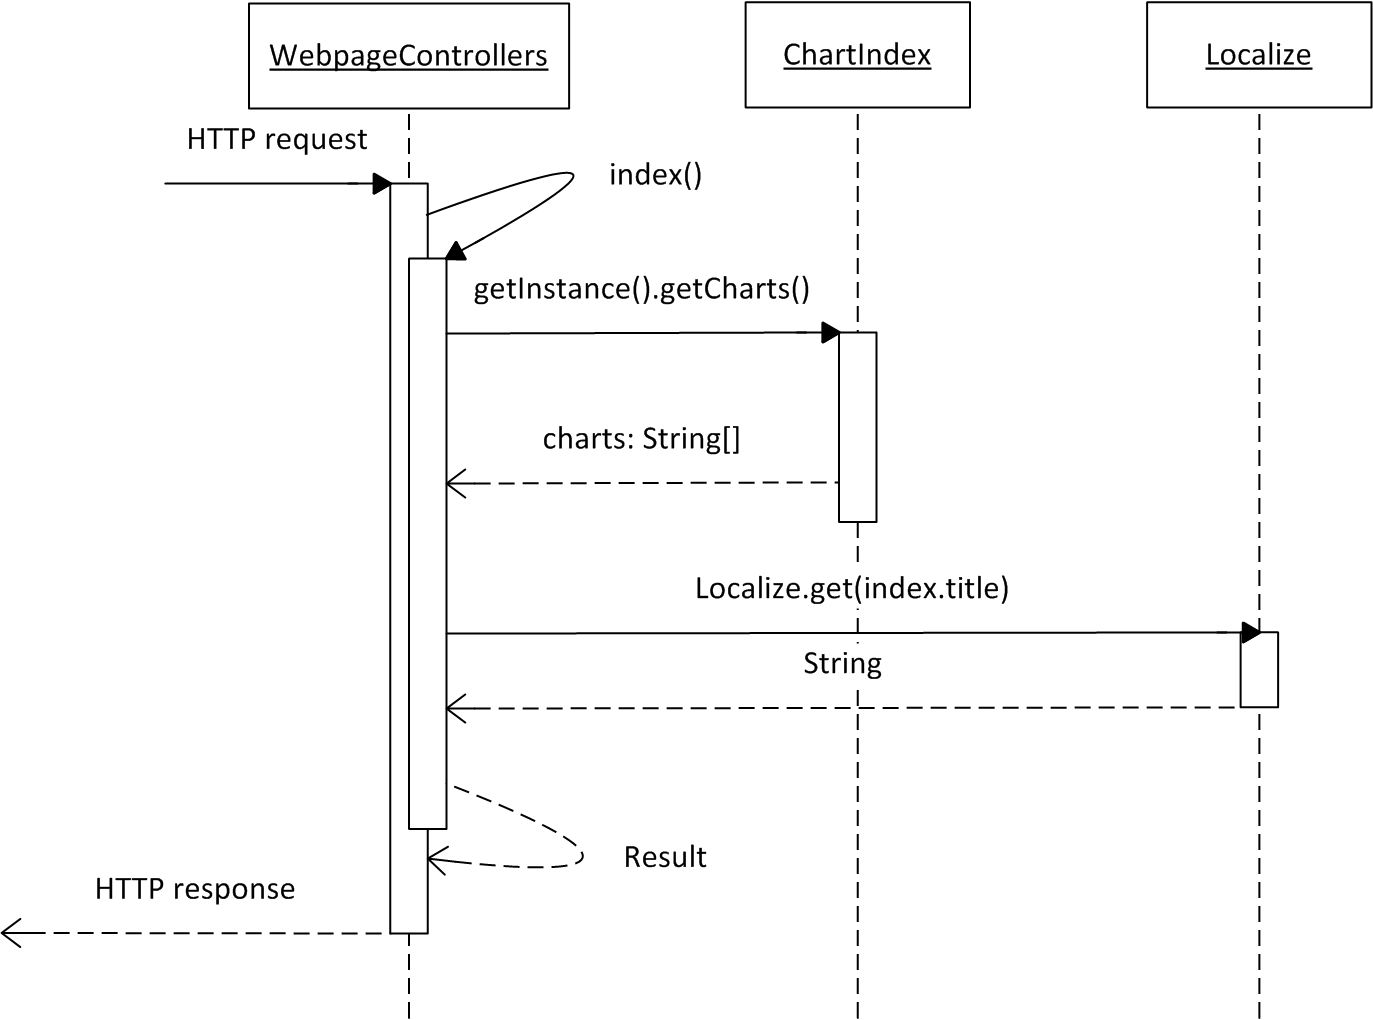
\includegraphics{Pictures/Seq/SeqHTTPRequest.png}
\end{center}


\newpage 
\subsection{Facade call}
In the following sequence diagram a call on the application tier facade is shown 
on the example of a chart request with \texttt{computeChart(..)}.

\begin{center}
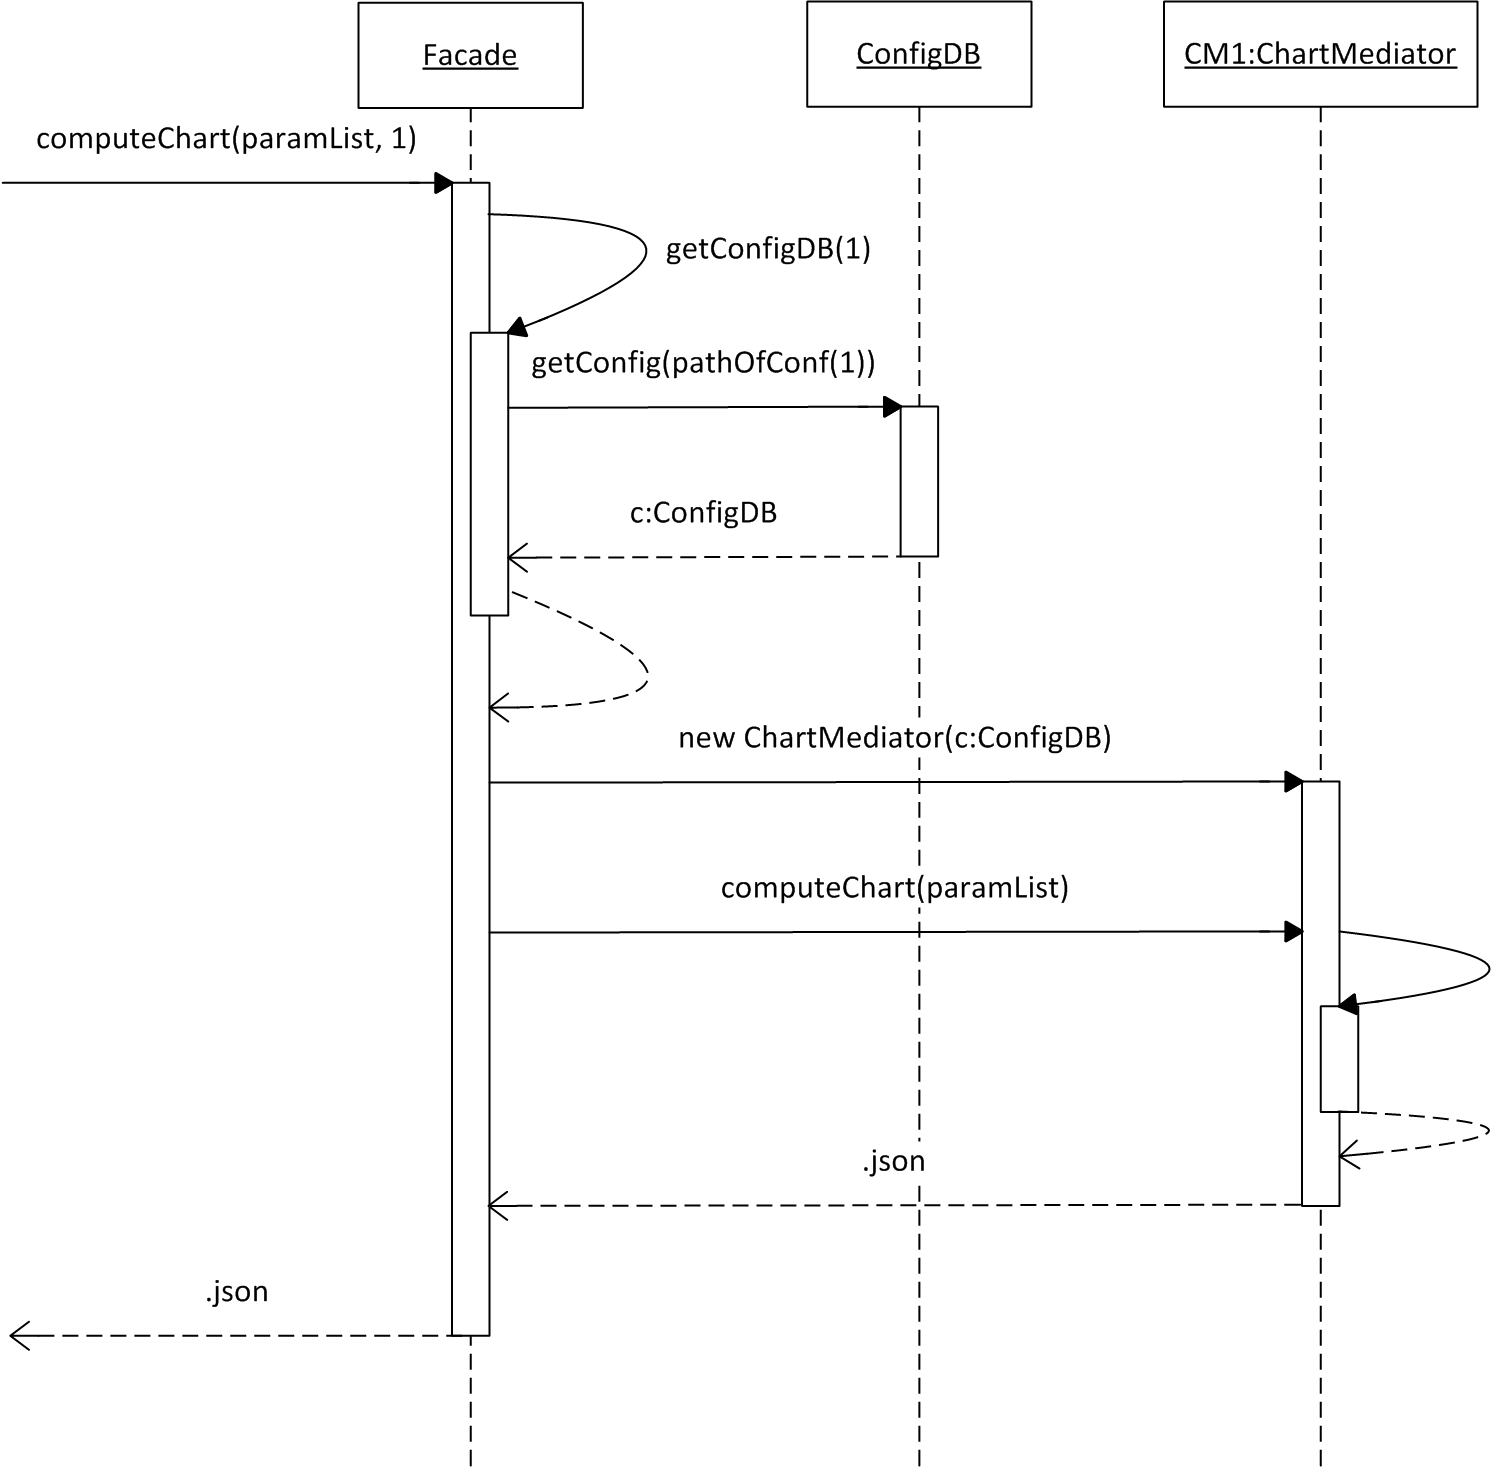
\includegraphics{Pictures/Seq/SeqFacade.png}  
\end{center} 
  


\newpage
\subsection{Chart request}
Sequence diagram of a \texttt{computeChart(..)} call, a chart request, on the ChartMediator.
 
\begin{center}
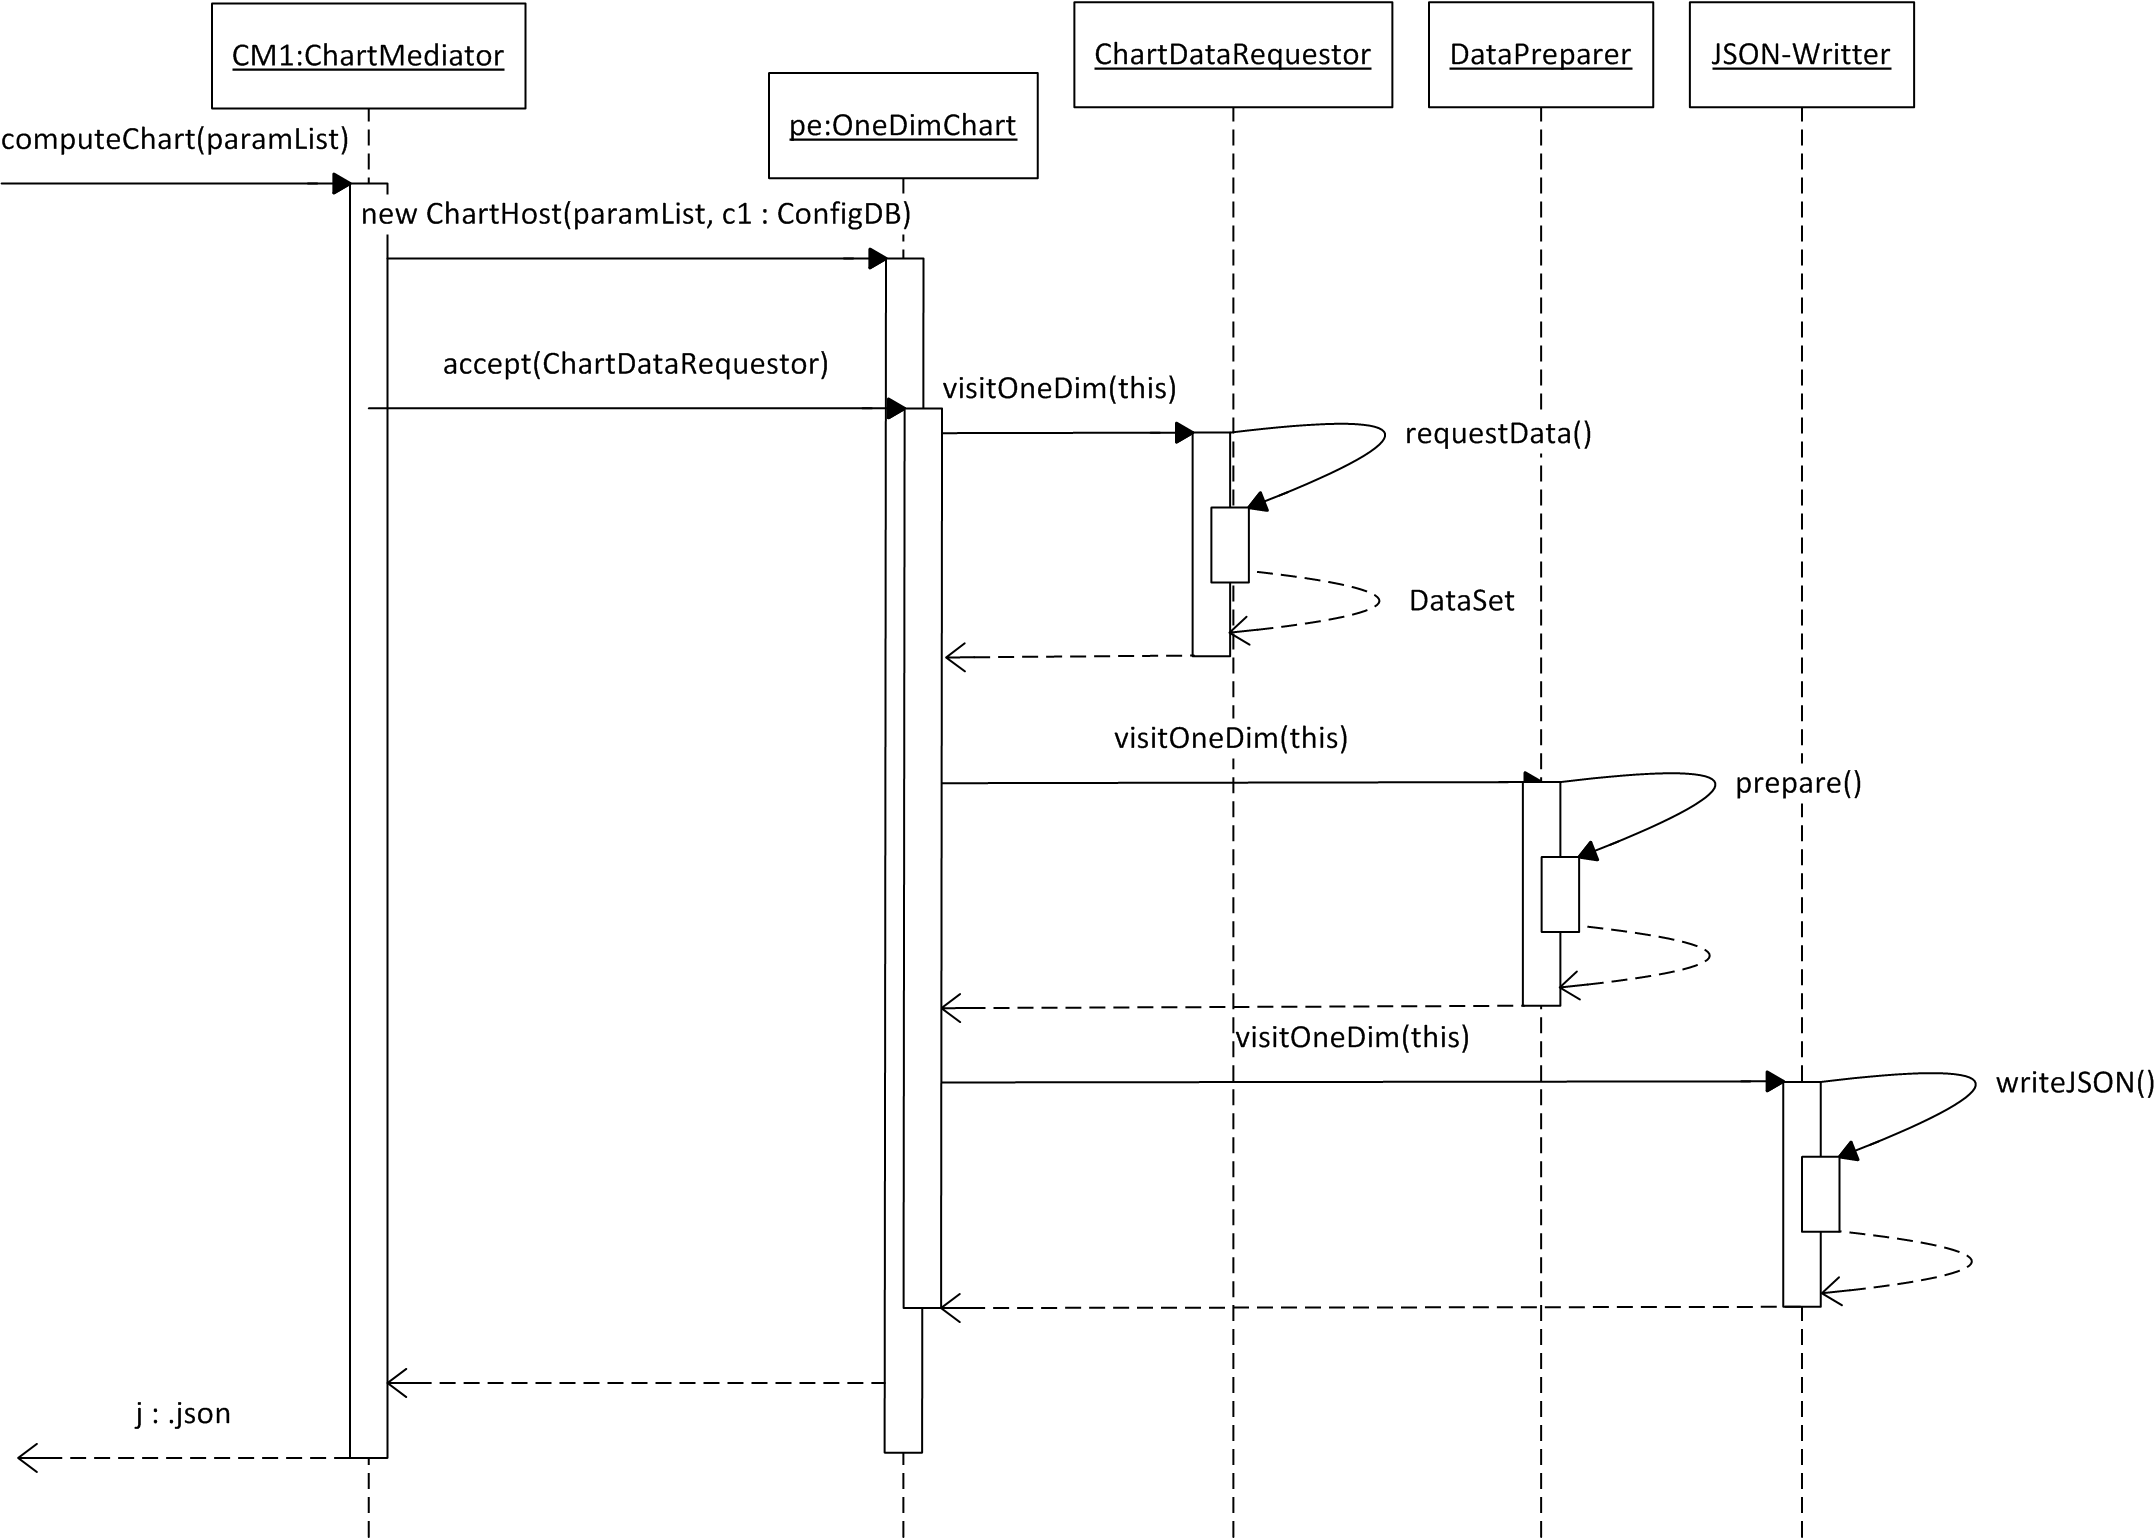
\includegraphics[width=1\linewidth]{Pictures/Seq/SeqChart.png}  
\end{center}
 
\newpage 

\subsection{Parsing} 
%This activity diagram shows the generall work flow of the parsing process of a log file. 
This sequence diagram describes the process after a ParsingTask for one line was created and
called with \texttt{run()}. 
% with the point of view on class interaction.

\begin{center}
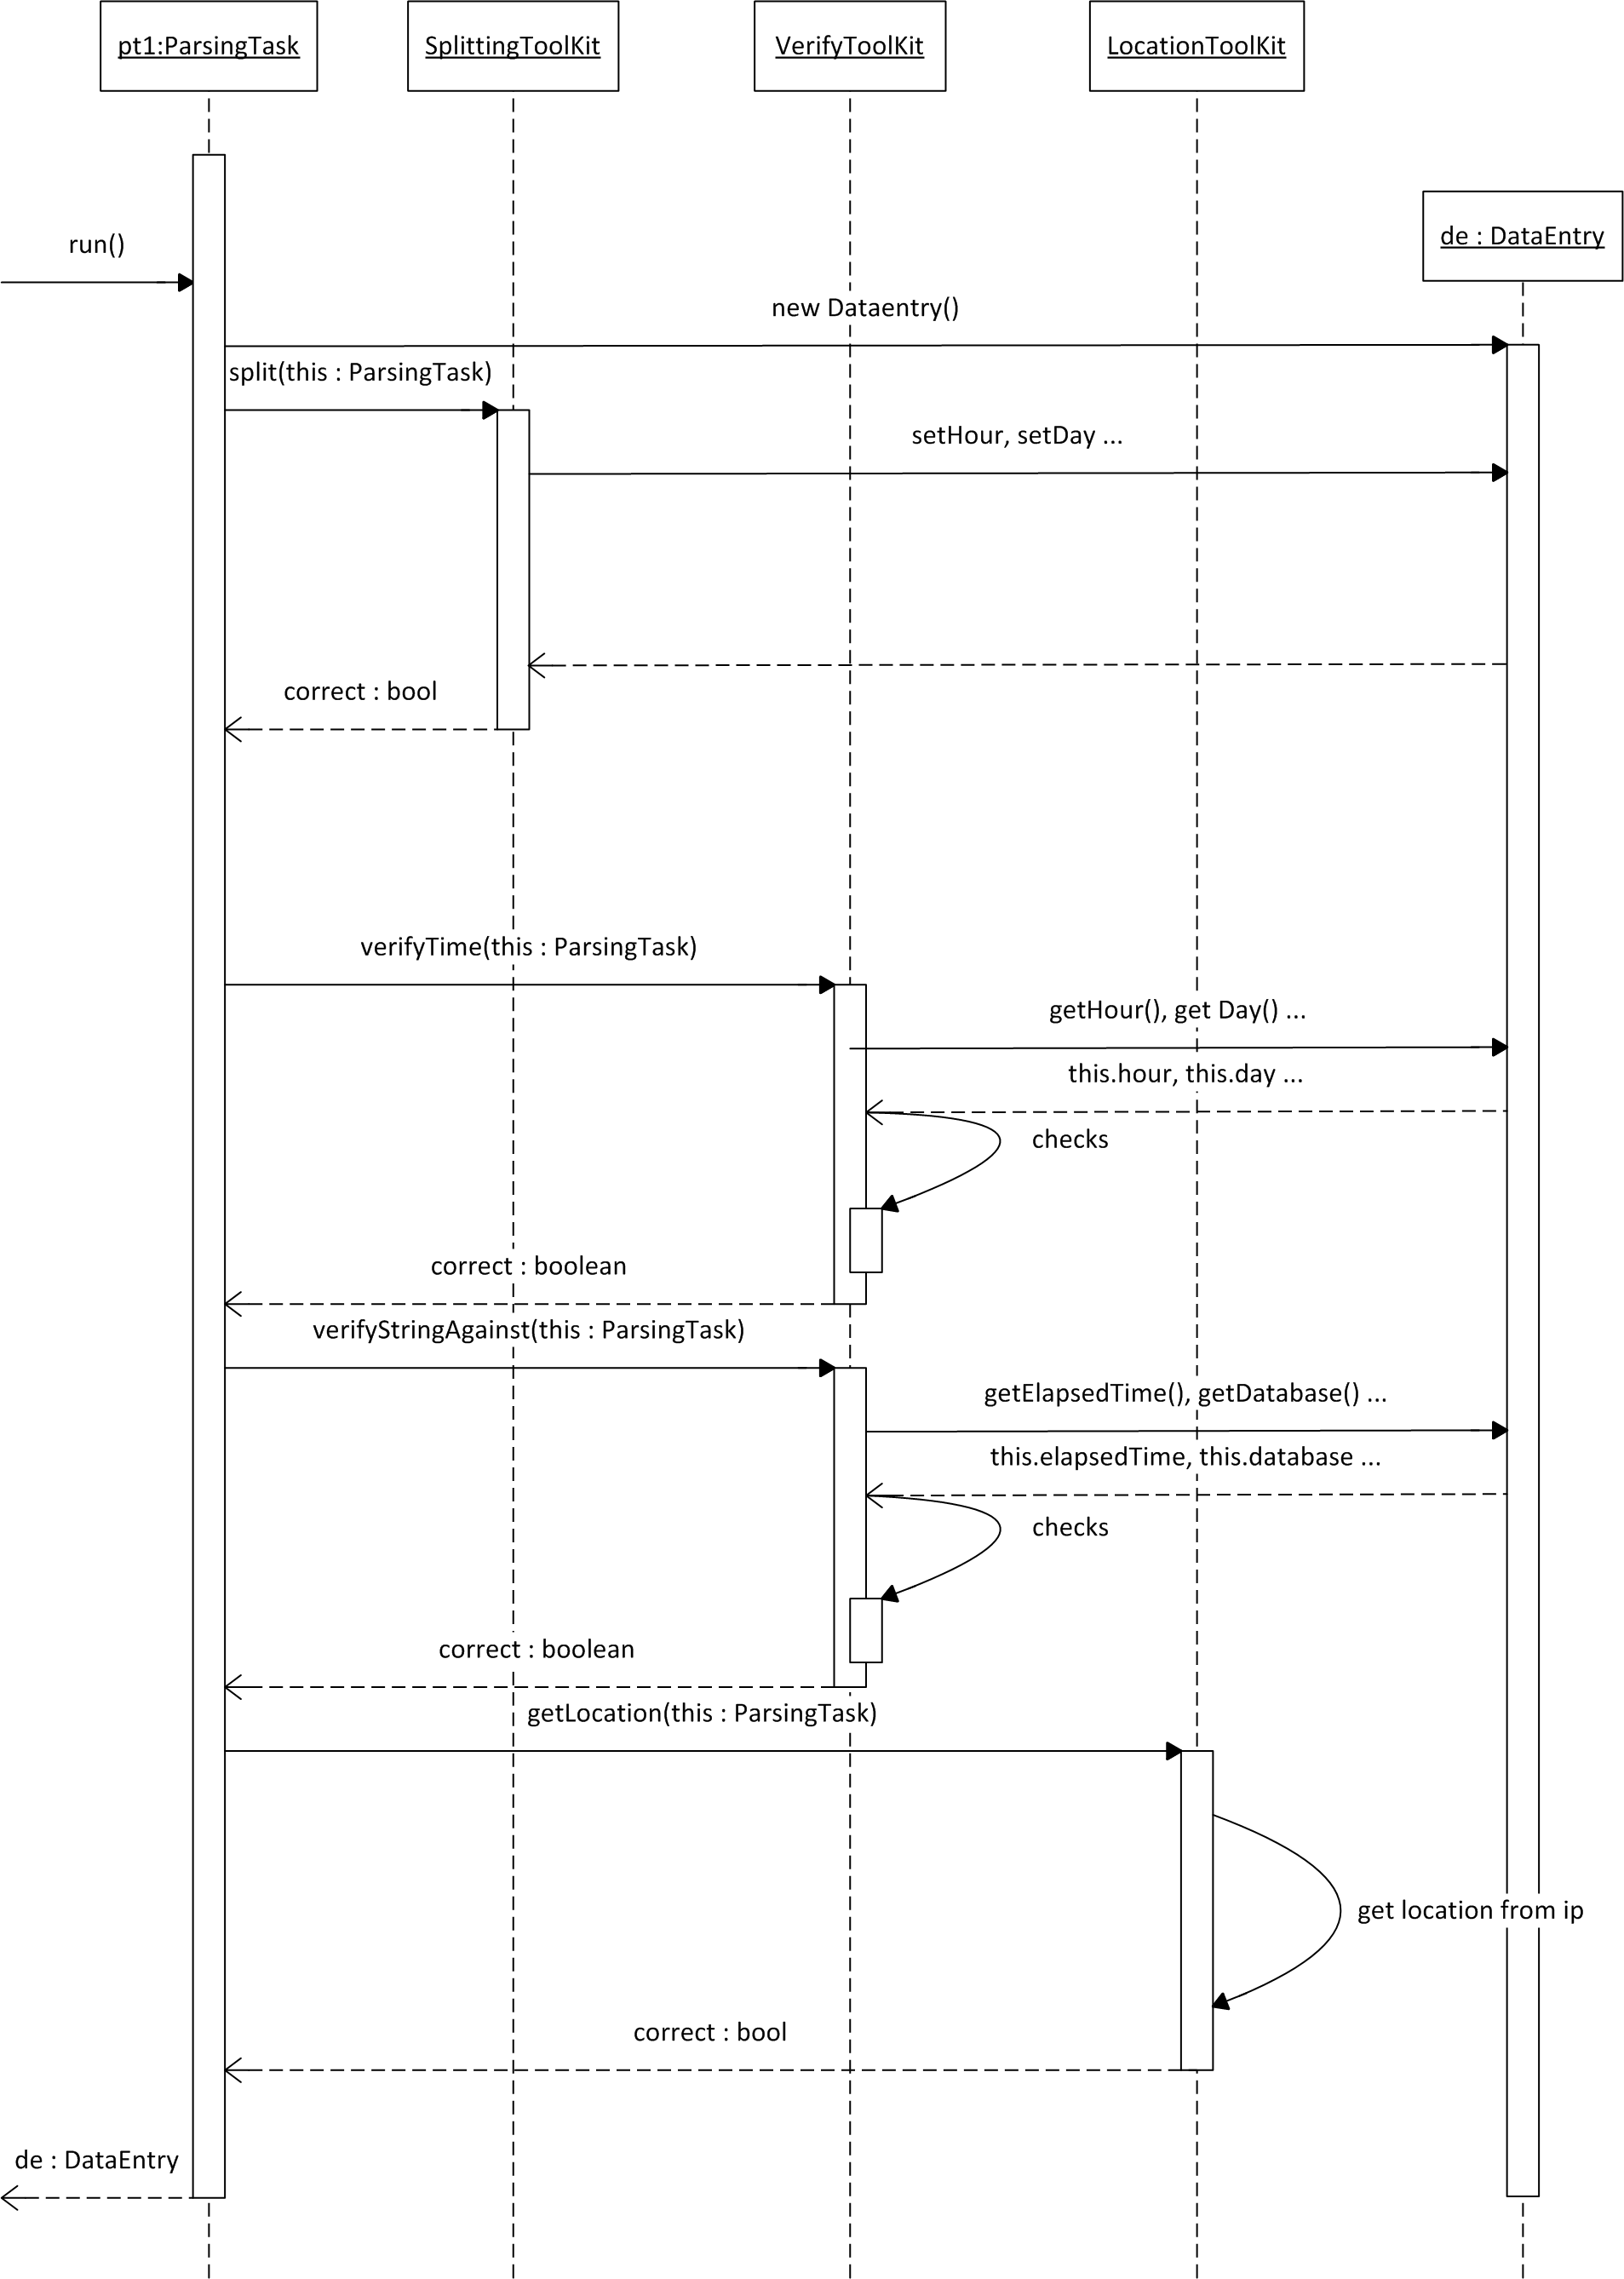
\includegraphics[width=0.8\linewidth]{Pictures/Seq/SeqParser.png}
\end{center}



    
